%% bare_jrnl.tex
%% V1.4b
%% 2015/08/26
%% by Michael Shell
%% see http://www.michaelshell.org/
%% for current contact information.
%%
%% This is a skeleton file demonstrating the use of IEEEtran.cls
%% (requires IEEEtran.cls version 1.8b or later) with an IEEE
%% journal paper.
%%
%% Support sites:
%% http://www.michaelshell.org/tex/ieeetran/
%% http://www.ctan.org/pkg/ieeetran
%% and
%% http://www.ieee.org/

%%*************************************************************************
%% Legal Notice:
%% This code is offered as-is without any warranty either expressed or
%% implied; without even the implied warranty of MERCHANTABILITY or
%% FITNESS FOR A PARTICULAR PURPOSE!
%% User assumes all risk.
%% In no event shall the IEEE or any contributor to this code be liable for
%% any damages or losses, including, but not limited to, incidental,
%% consequential, or any other damages, resulting from the use or misuse
%% of any information contained here.
%%
%% All comments are the opinions of their respective authors and are not
%% necessarily endorsed by the IEEE.
%%
%% This work is distributed under the LaTeX Project Public License (LPPL)
%% ( http://www.latex-project.org/ ) version 1.3, and may be freely used,
%% distributed and modified. A copy of the LPPL, version 1.3, is included
%% in the base LaTeX documentation of all distributions of LaTeX released
%% 2003/12/01 or later.
%% Retain all contribution notices and credits.
%% ** Modified files should be clearly indicated as such, including  **
%% ** renaming them and changing author support contact information. **
%%*************************************************************************

% *** Authors should verify (and, if needed, correct) their LaTeX system  ***
% *** with the testflow diagnostic prior to trusting their LaTeX platform ***
% *** with production work. The IEEE's font choices and paper sizes can   ***
% *** trigger bugs that do not appear when using other class files.       ***                          ***
% The testflow support page is at:
% http://www.michaelshell.org/tex/testflow/

\documentclass[a4paper, journal]{IEEEtran}

\usepackage[utf8]{inputenc}
\usepackage[T1]{fontenc}
\usepackage{mathptmx}
\usepackage{textcomp}
\usepackage{multirow}
\usepackage{xcolor}
\definecolor{codegreen}{rgb}{0,0.6,0}
\definecolor{codepurple}{rgb}{0.58,0,0.82}
\usepackage{listings}
\lstdefinestyle{mystyle}{
	commentstyle=\color{codegreen},
	keywordstyle=\color{magenta},
	stringstyle=\color{codepurple},
	showspaces=false,
	showstringspaces=false,
	breaklines=true
}
\lstset{style=mystyle}
\usepackage{amsmath}
\usepackage{amssymb}
\usepackage{float}
\usepackage{caption}
\captionsetup{
	aboveskip=4pt,
	belowskip=12pt
}
\usepackage[hidelinks]{hyperref}
\hypersetup{
	colorlinks=false
}
\usepackage[style=ieee]{biblatex}
\bibliography{bibliography/biblio}
\setlength{\parindent}{0pt}
\setlength{\parskip}{1.5em}
\usepackage{import}
% figure support
\usepackage{xifthen}
\pdfminorversion=7
\usepackage{pdfpages}
\usepackage{transparent}
\newcommand{\incfig}[1]{%
	\def\svgwidth{\columnwidth}
	\import{./figures/}{#1.pdf_tex}
}
\pdfsuppresswarningpagegroup=1

\begin{document}
\hypersetup{pageanchor=false}
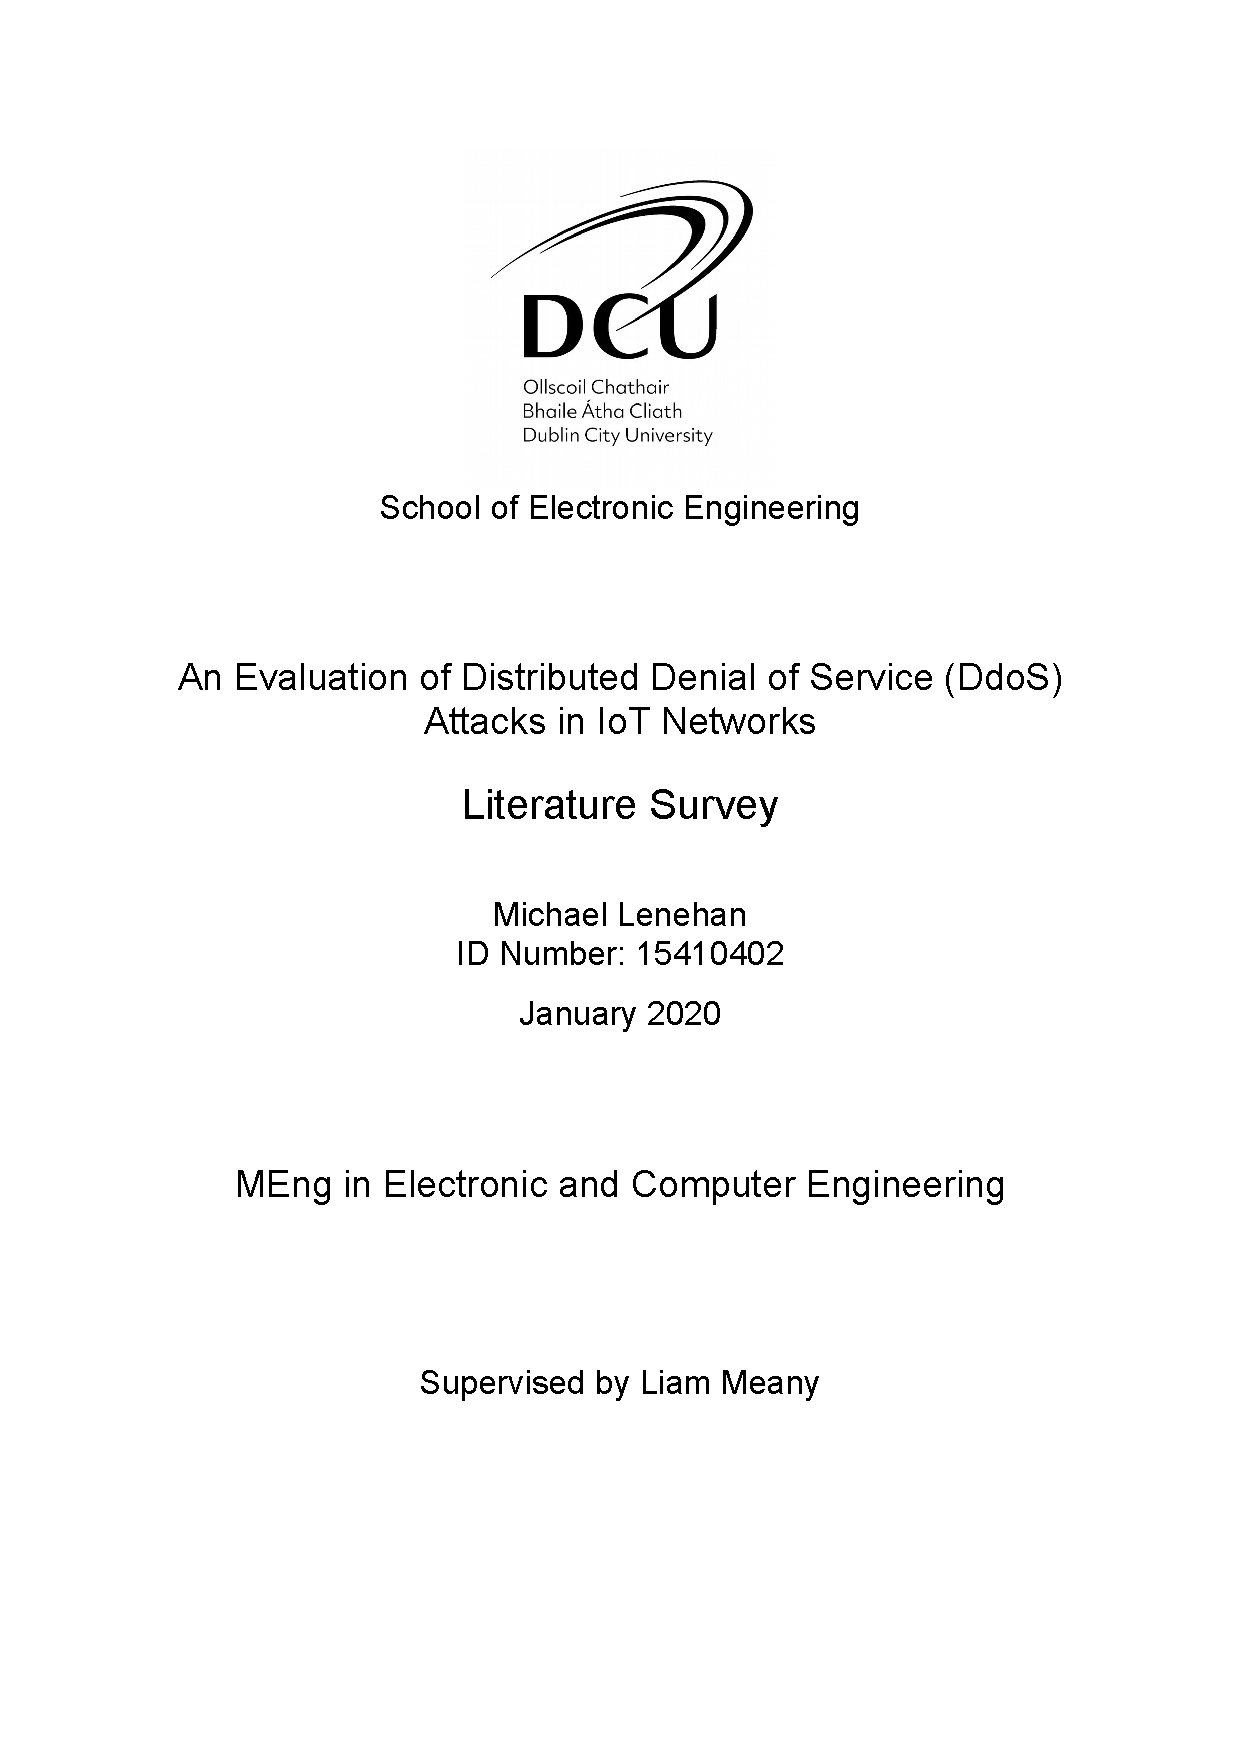
\includepdf[pages=-]{cover/coversheet}
\hypersetup{pageanchor=true}
\pagenumbering{arabic}
\title{An Evaluation of Distributed Denial of Service (DDoS) Attacks in IoT
Networks - Literature Review}
\author{Michael Lenehan}

\markboth{MEng in Electronic \& Computer Engineering, January 2020}%
{}

\maketitle

\begin{abstract}
	With the increase in the number of Internet of Things (IoT) connected devices
in recent years, and the projected growth in the number of connected devices in
the coming years, it is evident that there is a need to investigate the
security flaws which have made these devices a target for an increasing number
of Distributed Denial of
Service (DDoS) attacks. Following the Mirai botnet attack in 2016, it has become
apparent that there is much work required in securing IoT networks. Due to the
relatively low available resources in IoT devices, there is a need to implement
either non-resource intensive security features on the devices themselves, or to
implement more stringent security for these devices at the level of the network.

\end{abstract}

% Note that keywords are not normally used for peerreview papers.
\begin{IEEEkeywords}
	Internet of Things, Distributed Denial of Service, Security.
\end{IEEEkeywords}

\section{Introduction}
The aim of a Distributed Denial of Service attack is to disrupt the connection
between a service, such as an application server or DNS server, and that
services users.

Denial of Service (DoS) attacks typically exploited vulnerabilities with network
or application layer protocols, for example, Syn Floods or HTTP Floods. With these
types of attacks, spoofed IP addresses were typically used, both to mask the IP
address of the attacker, and to take advantage of vulnerabilities of the
protocols being used.

As DoS mitigation techniques improved, and attacks using IP spoofing became
easier to defend against, attackers began utilising botnets to perform
amplification attacks. Distributed Denial of Service (DDoS) attacks utilise
large number of hosts to perform attacks. These types of attacks prove more
difficult to defend against than typical Denial of Service attacks.

In order to extensively evaluate the impact of Distributed Denial of Service
attacks, and the role which IoT devices play in modern DDoS attacks, simulations
can be used. Simulations can show the impact to a network, and the disruption
caused by these attacks, without having to use real network devices.

\subsection{Simulation Software}

There were a number of simulation software packages considered for the tests
contained in this document. Each of these packages offer their own set of
advantages and disadvantages.

\subsubsection{ns-3}

The most commonly used network simulation software is "ns-3"; a "discrete-event
network simulator for Internet systems"\cite{nsnam_20AD}. This package is
commonly used for research purposes, and numerous examples of D/DoS simulations
implemented using ns-3 can be found\cite{}\cite{}.

\subsubsection{Cooja}

Another simulation software package considered was "Cooja". This package
simulates Wireless Sensor Networks built on the Contiki IoT operating
system\cite{cooja_2019}. While the underlying system being simulated is an IoT device,
there was little information to be found on implementing the types of testing
required, and as such this software package was ruled out.

\subsubsection{Mininet}

The final software package considered was "Mininet". Mininet is a network
simulator which uses Linux containers to emulate network
devices\cite{mininet_2018}. As the network devices are emulated using containers,
each host uses real Linux Kernel code.

As the Mininet hosts run Linux Kernel code, Linux applications can be easily
run. This is advantageous as common attack tools can be installed and executed.
Each host can be assigned a unique IP address allowing the attacking host to
address it's target as in a real attack situation. As each host is implemented
as a container, a terminal can be open for each host for manual command execution.

Mininet implements Software Defined Networking using the OpenFlow protocol. By
default, Mininet uses the OpenFlow reference controller, however, it also allows
for the use of remote controllers. The "Floodlight" controller will be used for
this purpose, as it has a GUI application which can display the network
topology.

Mininet virtualizes the network links between each host or switch in the
network. These links can be assigned parameters such as a delay time on the
link, or a set bandwidth.

The Python API implemented by Mininet allows for the topology and the terminal
commands to be created and executed programmatically. The Python API will be
used in order to execute repeatable tests with reproducible results.

Due to the advantages offered by the Mininet simulation software package, this
will be the simulator of choice for testing. There are however a number of
disadvantages which must be noted\cite{mnov_2018}.

\begin{enumerate}
	\item Containers share the file system of the host, i.e. the desktop or
		VM on which Mininet is being run
	\item A network cannot exceed the bandwidth of a single server
	\item Non-Linux-compatible OpenFlow switches and applications are not
		supported
\end{enumerate}

While these limitations must be kept in mind, they will not prove to be a
hindrance for the purposes of these simulations.


\section{Review and Analysis of Prior Work}
Salim et al.\cite{Salim2019} have presented a thorough survey of a number of different DDoS
attacks which are common in IoT networks. Their work provides classifications
for these attacks, along with providing a number of detection, prevention and
mitigation solutions.

\begin{figure}[H]
	\centering
	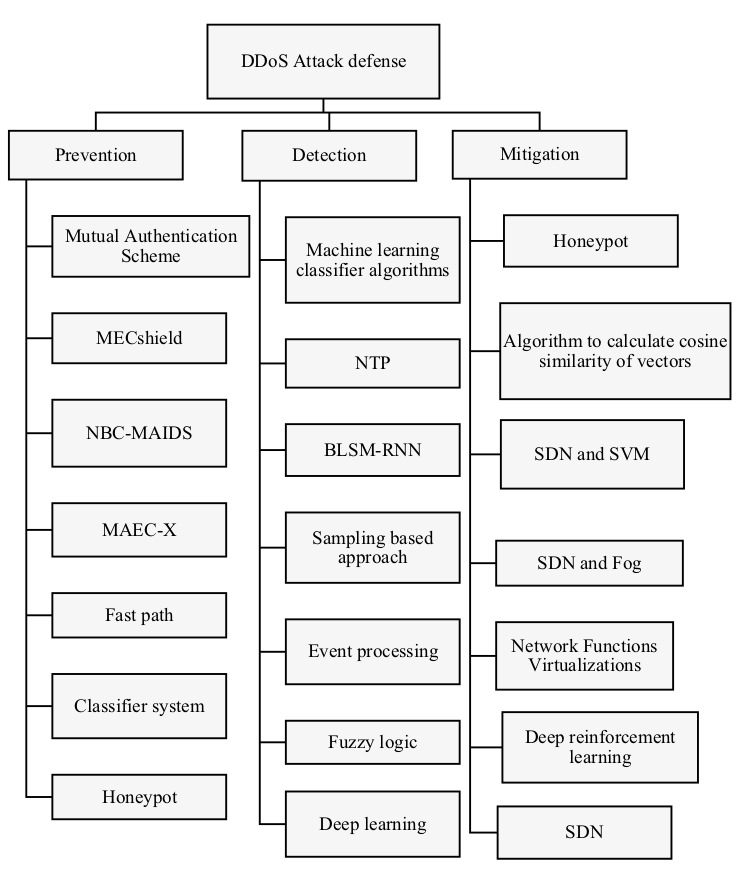
\includegraphics[width=0.5\textwidth]{images/salimDefenseDiagram.png}
	\caption{Salim et al. DDoS attack Defence techniques\cite{Salim2019}}
	\label{fig:salimDefense}
\end{figure}

As seen in Figure \ref{fig:salimDefense}, there are 21 proposed solutions; 7
Prevention, 7 Detection, and 7 Mitigation. These solutions act at the device
level, edge computing level, and cloud level.

Prevention of attacks deals in stopping traffic flow between nodes flagged for
suspicious or ``abnormal'' traffic. These techniques involve
monitoring the traffic between the nodes, and either stopping data flow (Mutual
Authentication Scheme), highlighting suspicious traffic to other nodes in the
network (MECshield, NBC-MAIDS, Multi-access Edge Computing, Fast Path,
Classifier System), or diverting attack traffic (Honeypot).

Detection of attacks deals in correctly detecting that the traffic flow is due
to an attack. These techniques utilise machine learning (Machine Learning
Classifier Algorithms, BLSM-RNN, Fuzzy Logic, Deep Learning) and event processing
(CEPID, Sampling-based Approach) in order to detect attack traffic, in some
cases, with very high accuracy. The Machine Learning Classifier Algorithms
technique had a recorded detection accuracy in real time IoT devices of 0.99\%.

Mitigation of attacks deals in stopping a detected DDoS attack. This attack
mitigation is implemented by blocking dataflow from malicious nodes within the
network (SDN and SVM, ECESID, Deep Reinforcement Learning, and SDN).


\section{Relation of Prior Work to the Project Problem}
test


\section{Conclusion}
The conclusion goes here.

%\vfill

\printbibliography

\end{document}
